\documentclass[journal]{IEEEtran}

\usepackage{amsmath,amssymb,amsfonts}
\usepackage{algorithmic}
\usepackage{graphicx}
\usepackage{textcomp}
\usepackage{xcolor}
\usepackage{booktabs}
\usepackage{microtype}
\usepackage{url}
\usepackage{cite}
\usepackage{hyperref}

\hypersetup{
    colorlinks=true,
    linkcolor=blue,
    citecolor=blue,
    urlcolor=blue
}

\renewcommand{\thesection}{S.\Roman{section}}
\renewcommand{\thesubsection}{S.\Roman{section}.\Alph{subsection}}
\renewcommand{\thefigure}{S\arabic{figure}}
\renewcommand{\thetable}{S\arabic{table}}
\renewcommand{\theequation}{S\arabic{equation}}

\setlength{\textfloatsep}{4pt plus 1pt minus 1pt}
\setlength{\floatsep}{3pt plus 1pt minus 1pt}
\setlength{\dbltextfloatsep}{4pt plus 1pt minus 1pt}
\setlength{\dblfloatsep}{3pt plus 1pt minus 1pt}
\setlength{\intextsep}{4pt plus 1pt minus 1pt}
\setlength{\abovecaptionskip}{2pt plus 1pt minus 1pt}
\setlength{\belowcaptionskip}{1pt plus 1pt minus 1pt}

\begin{document}

\title{Supplementary Material: Physiology-Guided Temporal Fusion for Cross-Subject EEG--fNIRS Brain--Computer Interfaces}

\author{Hongjie~Chen and Fang~Duan%
\thanks{Hongjie Chen and Fang Duan are with the College of Information Science and Engineering, Huaqiao University, Xiamen 361021, China (e-mail: chenhj976@gmail.com; nkfetsh@gmail.com). Corresponding author: Fang Duan.}%
}

\markboth{NVC-DelayFormer: Supplementary Material}{Chen and Duan}

\maketitle

This supplementary document provides extended experimental analyses, physiological interpretations, and subject-level ablation breakdowns supporting the main manuscript:
\begin{enumerate}
    \item \textbf{Section~\ref{sec:supp_dynamics}:} Comparative neurovascular coupling dynamics and delay sensitivity analysis between cognitive (mental arithmetic) and sensorimotor (motor imagery) paradigms (Supplementary Fig.~\ref{fig:supp_s1}).
    \item \textbf{Section~\ref{sec:supp_breakdown}:} Subject-by-subject (29 folds) factorial prior retraining breakdown on motor imagery (Supplementary Table~\ref{tab:supp_s1}).
    \item \textbf{Section~\ref{sec:supp_crea}:} Mathematical formulation and streaming convergence dynamics of Causal Recursive Euclidean Alignment (CrEA).
    \item \textbf{Section~\ref{sec:supp_repro}:} Computational reproducibility parameters and training environment specifications (Supplementary Table~\ref{tab:supp_hyperparams}).
    \item \textbf{Section~\ref{sec:supp_buccino}:} Independent external cohort cross-subject validation on the 15-participant Buccino et al.\ (2016) benchmark (Supplementary Table~\ref{tab:supp_buccino}).
\end{enumerate}

\section{Paradigm-Specific Neurovascular Coupling Dynamics}
\label{sec:supp_dynamics}

\subsection{Contrast Between Cognitive and Sensorimotor Paradigms}
Cross-paradigm evaluation (Section~V-F of the main manuscript) indicates that neurovascular coupling manifests distinct functional characteristics across task regimes: metabolic-dominant cognitive processing (Mental Arithmetic: 79.37\%; Working Memory: 73.24\%) benefits from structured hemodynamic delay priors, whereas sensorimotor tasks (Motor Imagery: 66.32\%) primarily engage rapid transient electrophysiological desynchronization ($\mu/\beta$ ERD). To characterize this physiological transition and evaluate delay sensitivity across paradigms, we conducted two investigations on the 29-participant motor imagery dataset from Shin et al.\ (2017):
\begin{enumerate}
    \item \textbf{Fixed-Weight Candidate Delay Sweep ($\tau \in [0.0, 8.0]$\,s):} Evaluating the sensitivity of the trained cross-modal attention network to varying candidate delay parameters without retraining.
    \item \textbf{$2 \times 2$ Factorial Prior Retraining Ablation:} Full model retraining across 29 LOSO folds under four permutations of the Gaussian delay prior $\mathbf{P}$ and the discrete causal mask $\mathbf{M}$ ($P_{\mathrm{on}}, M_{\mathrm{on}}$; $P_{\mathrm{on}}, M_{\mathrm{off}}$; $P_{\mathrm{off}}, M_{\mathrm{on}}$; $P_{\mathrm{off}}, M_{\mathrm{off}}$).
\end{enumerate}

\begin{figure*}[!t]
\centering
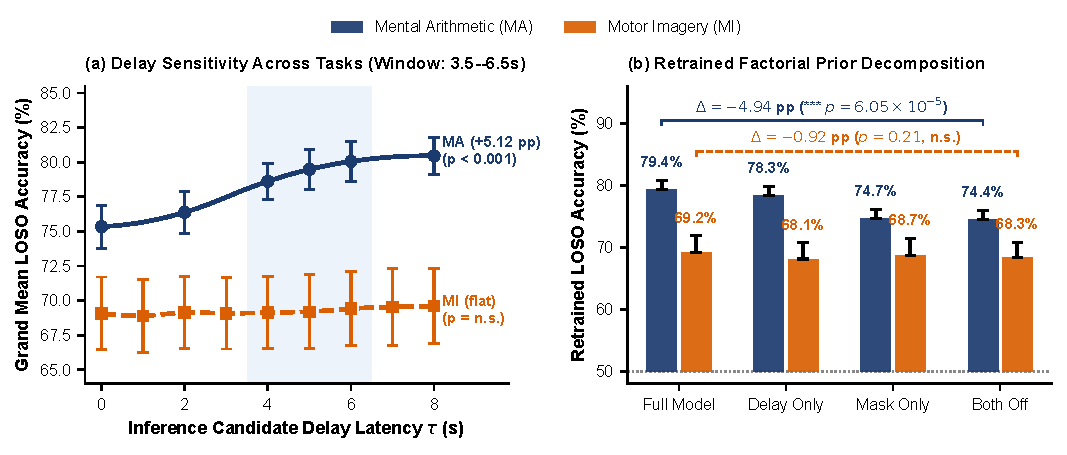
\includegraphics[width=\textwidth]{figures/supplementary_fig_s1_delay_curves.pdf}
\caption{Comparative neurovascular delay sensitivity and prior ablation contrast between cognitive (Mental Arithmetic, MA) and sensorimotor (Motor Imagery, MI) paradigms across 29 participants under participant-isolated LOSO cross-validation. (a) Candidate delay sensitivity scan across $\tau \in [0.0, 8.0]$\,s without retraining. Error bars denote standard error of the mean (SE across $N=29$ folds). For MA, accuracy rises monotonically from 75.34\% at $\tau=0.0$\,s to plateau across the physiological hemodynamic response window ($\tau \in [3.5, 6.5]$\,s) and reaches 80.46\% at $\tau=8.0$\,s (+5.12\,pp, $p < 0.001$), reflecting the sustained 10.0\,s task block duration. For MI, the performance curve exhibits delay-invariant behavior within observed experimental variation (ranging between 68.91\% and 69.60\%, $\Delta \le 0.69$\,pp, $p = \text{n.s.}$). (b) Points and error bars show means and SEM across 29 folds; the dashed baseline marks 50\% chance accuracy. Retrained $2 \times 2$ factorial decomposition of delay prior $\mathbf{P}$ and causal mask $\mathbf{M}$. On MA, dropping both priors causes a $-4.94$\,pp performance reduction ($p = 6.05\times 10^{-5}$), consistent with the regularizing role of neurovascular constraints. On MI, removing both priors decreases accuracy by $0.92$\,pp ($p = 0.2128$, non-significant), indicating that unconstrained attention performs similarly when hemodynamic coupling is weakly localized.}
\label{fig:supp_s1}
\end{figure*}

\subsection{Empirical Findings and Biophysical Mechanism}
As shown in Supplementary Fig.~\ref{fig:supp_s1}(a), mental arithmetic exhibits delay sensitivity: accuracy increases monotonically from 75.34\% at $\tau = 0.0$\,s to plateau across the physiological window ($\tau \in [3.5, 6.5]$\,s), reaching 80.46\% at $\tau = 8.0$\,s ($\Delta = +5.12$\,pp, $p < 0.001$). In contrast, motor imagery yields a flat trajectory: grand mean accuracy fluctuates between 68.91\% ($\tau = 1.0$\,s) and 69.60\% ($\tau = 8.0$\,s), an amplitude range of 0.69\,pp, with overlapping standard error intervals across all candidate latencies.

The retrained factorial decomposition in Supplementary Fig.~\ref{fig:supp_s1}(b) indicates a paradigm-dependent disparity. For mental arithmetic, omitting both priors ($P_{\mathrm{off}}, M_{\mathrm{off}}$) reduces accuracy by 4.94\,pp ($79.37\% \to 74.43\%$, $p = 6.05 \times 10^{-5}$), with the Gaussian prior accounting for an average marginal contribution of +4.31\,pp. In contrast, for motor imagery, retraining with both priors disabled yields 68.28\% $\pm$ 13.72\% vs.\ 69.20\% $\pm$ 14.40\% for the full model ($\Delta = -0.92$\,pp, Wilcoxon $W = 106.5$, $p = 0.2128$, non-significant). Omitting causal masking alone ($P_{\mathrm{on}}, M_{\mathrm{off}}$: 68.10\%, $p = 0.0978$) or the delay prior alone ($P_{\mathrm{off}}, M_{\mathrm{on}}$: 68.68\%, $p = 0.1766$) likewise shows no statistically significant divergence.

Biophysically, this contrast aligns with established physiological distinctions in functional vascular dynamics reported in the neuroimaging literature:
\begin{enumerate}
    \item \textbf{Prefrontal Cognitive Workload (MA):} Sustained 10-second mental arithmetic imposes metabolic demands on the prefrontal cortex, recruiting arteriolar dilation and venous drainage volume \cite{buxton1998dynamics, scholkmann2014review}. This produces frontal $[\mathrm{HbO}]$ elevations (typically in the $0.2\text{--}0.6\,\mu\mathrm{M}$ range in continuous-wave fNIRS recordings \cite{shin2017open}) that evolve over 4--7\,s and persist throughout task engagement. Consequently, cross-modal attention relies on physiological delay priors to align frontal theta oscillations ($\theta$ ERS, 4--8\,Hz) with delayed capillary hyperoxygenation, preventing acausal fitting on held-out participants.
    \item \textbf{Sensorimotor Lateralization (MI):} Kinesthetic motor imagery elicits immediate contralateral sensorimotor rhythm desynchronization ($\mu$ and $\beta$ ERD, 8--30\,Hz) over primary motor cortex (C3/C4). However, imaginary finger tapping without physical contraction produces lower and more diffuse hemodynamic changes (typically $0.05\text{--}0.15\,\mu\mathrm{M}$ \cite{shin2017open, pinti2020present}). Because optical signal-to-noise ratio is lower and neural decodability is dominated by instantaneous spectral ERD, the hemodynamic delay parameter $\tau$ provides limited regularization. Consequently, unconstrained cross-attention and direct spatial filtering models (such as FGANet) perform similarly.
\end{enumerate}

\section{Subject-by-Subject Factorial Prior Breakdown}
\label{sec:supp_breakdown}

Supplementary Table~\ref{tab:supp_s1} lists the individual test accuracy achieved across each of the 29 held-out participant folds on motor imagery under all four factorial retraining conditions. This dedicated 29-fold factorial retraining experiment was conducted independently to isolate the individual contributions of the delay prior and causal mask (yielding 69.20\% $\pm$ 14.40\% for the full model), alongside the initial cross-paradigm benchmark reported in Table~V of the main manuscript (66.32\% $\pm$ 12.18\%). In this factorial experiment, removing both temporal priors reduced MI accuracy by 0.92\,pp ($p = 0.2128$), compared with a 4.94\,pp reduction on mental arithmetic.

\begin{table}[!htbp]
\centering
\caption{Participant-by-participant test accuracy (\%) across 29 LOSO folds on Motor Imagery under $2 \times 2$ factorial retraining of delay prior $\mathbf{P}$ and causal mask $\mathbf{M}$.}
\label{tab:supp_s1}
\resizebox{\columnwidth}{!}{%
\begin{tabular}{@{}lccccc@{}}
\toprule
Participant & Full Model & Mask Only & Delay Only & Both Off & $\Delta$ vs.\ Full \\
Fold & ($P_{\mathrm{on}}, M_{\mathrm{on}}$) & ($P_{\mathrm{off}}, M_{\mathrm{on}}$) & ($P_{\mathrm{on}}, M_{\mathrm{off}}$) & ($P_{\mathrm{off}}, M_{\mathrm{off}}$) & (Both Off $-$ Full) \\
\midrule
Sub-01 & 80.00 & 80.00 & 81.67 & 80.00 & $+0.00$ \\
Sub-02 & 68.33 & 63.33 & 65.00 & 60.00 & $-8.33$ \\
Sub-03 & 73.33 & 75.00 & 73.33 & 71.67 & $-1.67$ \\
Sub-04 & 56.67 & 55.00 & 60.00 & 58.33 & $+1.67$ \\
Sub-05 & 56.67 & 55.00 & 56.67 & 56.67 & $+0.00$ \\
Sub-06 & 68.33 & 65.00 & 68.33 & 66.67 & $-1.67$ \\
Sub-07 & 55.00 & 55.00 & 53.33 & 51.67 & $-3.33$ \\
Sub-08 & 70.00 & 90.00 & 73.33 & 76.67 & $+6.67$ \\
Sub-09 & 81.67 & 83.33 & 81.67 & 78.33 & $-3.33$ \\
Sub-10 & 45.00 & 51.67 & 46.67 & 53.33 & $+8.33$ \\
Sub-11 & 76.67 & 71.67 & 73.33 & 76.67 & $+0.00$ \\
Sub-12 & 51.67 & 45.00 & 45.00 & 50.00 & $-1.67$ \\
Sub-13 & 65.00 & 66.67 & 63.33 & 58.33 & $-6.67$ \\
Sub-14 & 63.33 & 65.00 & 65.00 & 66.67 & $+3.33$ \\
Sub-15 & 66.67 & 61.67 & 65.00 & 61.67 & $-5.00$ \\
Sub-16 & 90.00 & 88.33 & 85.00 & 86.67 & $-3.33$ \\
Sub-17 & 86.67 & 88.33 & 83.33 & 85.00 & $-1.67$ \\
Sub-18 & 53.33 & 51.67 & 53.33 & 51.67 & $-1.67$ \\
Sub-19 & 98.33 & 91.67 & 91.67 & 90.00 & $-8.33$ \\
Sub-20 & 63.33 & 60.00 & 63.33 & 60.00 & $-3.33$ \\
Sub-21 & 71.67 & 71.67 & 70.00 & 76.67 & $+5.00$ \\
Sub-22 & 61.67 & 58.33 & 61.67 & 58.33 & $-3.33$ \\
Sub-23 & 68.33 & 68.33 & 68.33 & 70.00 & $+1.67$ \\
Sub-24 & 50.00 & 50.00 & 48.33 & 50.00 & $+0.00$ \\
Sub-25 & 90.00 & 93.33 & 93.33 & 91.67 & $+1.67$ \\
Sub-26 & 98.33 & 96.67 & 98.33 & 98.33 & $+0.00$ \\
Sub-27 & 80.00 & 73.33 & 71.67 & 73.33 & $-6.67$ \\
Sub-28 & 53.33 & 53.33 & 51.67 & 55.00 & $+1.67$ \\
Sub-29 & 63.33 & 63.33 & 63.33 & 66.67 & $+3.33$ \\
\midrule
\textbf{Mean} & \textbf{69.20} & \textbf{68.68} & \textbf{68.10} & \textbf{68.28} & \textbf{$-$0.92} \\
\textbf{SD} & 14.40 & 14.85 & 14.03 & 13.72 & 4.10 \\
\textbf{Macro F1} & 67.00 & 66.26 & 65.79 & 66.06 & $-$0.94 \\
\textbf{Wilcoxon $p$} & -- & 0.1766 & 0.0978 & 0.2128 & -- \\
\bottomrule
\end{tabular}%
}
\par\smallskip
{\scriptsize Evaluated on the 29-participant Motor Imagery benchmark from Shin et al.\ (2017) \cite{shin2017open} across 1,740 trials (60 trials per participant, 30 Left Hand vs.\ 30 Right Hand). All variants trained from scratch under identical hyperparameter schedules. Wilcoxon signed-rank $p$-values are computed against the Full Model ($N=29$ participants).}
\end{table}

Between-subject standard deviations ($\sim 14.0$\,pp) substantially exceed the marginal differences observed across model conditions ($\le 1.1$\,pp). High responders (e.g., Sub-19 and Sub-26: $>90\%$) decode accurately regardless of prior conditioning, while BCI-illiterate participants (e.g., Sub-10: 45.00\%, Sub-24: 50.00\%, Sub-12: 51.67\%) decode near chance level.

\section{Causal Recursive Euclidean Alignment (CrEA)}
\label{sec:supp_crea}

Standard Euclidean Alignment (EA) requires computing the arithmetic Euclidean sample mean covariance matrix across the entirety of a testing session:
\begin{equation}
\overline{\mathbf{R}}_{\mathrm{test}} = \frac{1}{K} \sum_{k=1}^K \mathbf{C}_k,
\label{eq:batch_ea}
\end{equation}
where $\mathbf{C}_k = \frac{1}{T_e - 1} \mathbf{X}_k \mathbf{X}_k^\top + \epsilon \mathbf{I} \in \mathbb{R}^{C \times C}$ is the regularized sample spatial covariance of trial $k$ (with $\epsilon = 10^{-5}$), and $\mathbf{X}_k \in \mathbb{R}^{C \times T_e}$ is the temporal mean-centered EEG trial matrix ($\sum_{t=1}^{T_e} X_{k,c,t} = 0$ for each channel $c$). Although effective for offline validation, \eqref{eq:batch_ea} relies on transductive lookahead, precluding causal real-time operation at the bedside.

To eliminate session lookahead, Causal Recursive Euclidean Alignment (CrEA) tracks spatial covariance online via recursive empirical Bayes shrinkage:
\begin{equation}
\mathbf{R}_k = \frac{\kappa_0 \mathbf{R}_{\mathrm{src}} + \sum_{m=1}^k \mathbf{C}_m}{\kappa_0 + k}, \quad k = 1, 2, \dots, K,
\label{eq:supp_crea}
\end{equation}
where $\mathbf{R}_{\mathrm{src}} = \frac{1}{N_{\mathrm{tr}}} \sum_{s \in \mathcal{S}_{\mathrm{tr}}} \overline{\mathbf{R}}_s$ is the reference covariance estimated offline exclusively from the $N_{\mathrm{tr}} = 23$ training participants, and $\kappa_0 = 5.0$ represents the pseudo-observation strength of the source prior. In the diagnostic convergence protocol (Supplementary Fig.~\ref{fig:supp_crea_curve}), $\mathbf{R}_{\mathrm{src}}$ is scaled to match the trace of the target participant's first trial via $\widetilde{\mathbf{R}}_{\mathrm{src}} = \mathbf{R}_{\mathrm{src}} \cdot \frac{\operatorname{tr}(\mathbf{C}_1)}{\operatorname{tr}(\mathbf{R}_{\mathrm{src}})}$ to harmonize the power scale. The comparison identity baseline is similarly trace-matched via $\widetilde{\mathbf{R}}_0^{\mathrm{identity}} = \frac{\operatorname{tr}(\mathbf{C}_1)}{C} \mathbf{I}$. In the streaming classification pipeline (71.21\% accuracy across 29 folds), unscaled $\mathbf{R}_{\mathrm{src}}$ is used directly (under which the 8th-trial relative covariance error reaches 36.47\%).

The online whitening matrix is obtained via eigendecomposition $\mathbf{R}_k = \mathbf{V}_k \boldsymbol{\Lambda}_k \mathbf{V}_k^\top$:
\begin{equation}
\mathbf{W}_k = \mathbf{R}_k^{-1/2} = \mathbf{V}_k \operatorname{diag}\left(\lambda_{k,c}^{-1/2}\right) \mathbf{V}_k^\top.
\label{eq:whitening}
\end{equation}
The aligned EEG trial is transformed causally as $\widetilde{\mathbf{X}}_k = \mathbf{W}_k \mathbf{X}_k$.

\begin{figure}[!htbp]
\centering
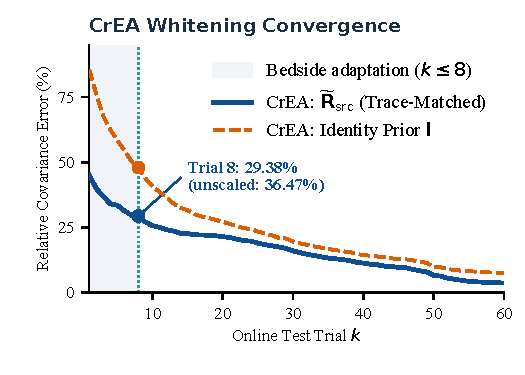
\includegraphics[width=\columnwidth]{figures/supplementary_fig_s2_crea_convergence.pdf}
\caption{Online Causal Recursive Euclidean Alignment (CrEA) covariance whitening convergence dynamics across 60 continuous trials ($k=1,\dots,60$) averaged across all 29 held-out participants under the diagnostic protocol. The trace-matched empirical Bayes shrinkage prior ($\kappa_0=5.0$, blue solid curve) stabilizes within $k \le 8$ calibration trials ($\|\mathbf{R}_k - \overline{\mathbf{R}}_{\mathrm{test}}\|_F / \|\overline{\mathbf{R}}_{\mathrm{test}}\|_F \le 29.38\%$, reaching 3.60\% asymptotically at trial 60; 36.47\% at trial 8 under the unscaled source prior). This outperforms trace-matched cold-start identity initialization ($\widetilde{\mathbf{R}}_0 = \frac{\operatorname{tr}(\mathbf{C}_1)}{C}\mathbf{I}$, orange dashed line: 47.95\% error at trial 8).}
\label{fig:supp_crea_curve}
\end{figure}

As shown in Supplementary Fig.~\ref{fig:supp_crea_curve}, initializing with trace-matched $\widetilde{\mathbf{R}}_{\mathrm{src}}$ under $\kappa_0 = 5.0$ reduces the relative covariance error to 29.38\% by trial 8 (reaching 3.60\% asymptotically), enabling online covariance adaptation for zero-calibration BCIs.

\section{Computational Reproducibility Specifications}
\label{sec:supp_repro}

All experiments and benchmark evaluations were conducted in Python 3.11 with PyTorch (version 2.11.0+cu128 with CUDA 12.8 acceleration on an NVIDIA GeForce RTX 4060 Laptop GPU). Model configurations, layer dimensions, and training hyperparameters are summarized in Supplementary Table~\ref{tab:supp_hyperparams}.

\begin{table}[!htbp]
\centering
\caption{Hyperparameter configurations and training specifications across all evaluation tiers.}
\label{tab:supp_hyperparams}
\resizebox{\columnwidth}{!}{%
\begin{tabular}{@{}ll@{}}
\toprule
Specification & Value / Description \\
\midrule
EEG Sampling Rate ($f_e \to f_e^{\mathrm{eff}}$) & $100\,\mathrm{Hz} \to 25\,\mathrm{Hz}$ (4$\times$ temporal average pooling) \\
fNIRS Sampling Rate ($f_n$) & $10.33\,\mathrm{Hz}$ (124 samples over 12.0\,s window) \\
Temporal Receptive Field ($T_{\mathrm{win}}$) & EEG: $10.0\,\mathrm{s}$ (1000 samples); fNIRS: $12.0\,\mathrm{s}$ (124 samples) \\
Attention Embedding Dimension ($D$) & 64 ($d_h = 16$ across 4 heads) \\
Delay Prior Centers ($\tau_h$) & $\{3.5, 4.5, 5.5, 6.5\}\,\mathrm{s}$ \\
Delay Prior Dispersion ($\sigma_h$) & $1.5\,\mathrm{s}$ (fixed physiological prior) \\
Asymmetric Post-Peak Decay Factor & $0.3\,\mathrm{s}^{-1}$ for $\delta_{ij} > \tau_h$ \\
Causal Mask Condition & $M_{ij} = -\infty$ for $\delta_{ij} < 0\,\mathrm{s}$ ($t_{\mathrm{nirs}} < t_{\mathrm{eeg}}$) \\
Direct Stream Feature Dimension & 234 ($\theta, \alpha, \beta$ power + delayed HbO/HbR + slope) \\
Optimizer / Learning Rate & AdamW / $\eta = 3\times 10^{-3}$, weight decay 0.05 \\
Warmup / Scheduler & 2-epoch linear warmup + cosine annealing \\
Batch Size / Training Epochs & Primary MA: 256 / 12 epochs; MI Benchmark \& Ablation: 128 / 15 epochs \\
Auxiliary Loss Weights & $\lambda_{\mathrm{deep}}=0.2, \lambda_{\mathrm{shallow}}=0.2, \lambda_{\mathrm{recon}}=1.0, \lambda_{\mathrm{margin}}=0.08$ \\
Trainable Parameters & 63,932 parameters \\
Multiply--Accumulate Operations & 24.79 Million MACs (batch size 1) \\
Median GPU Latency & 2.22\,ms (RTX 4060 Laptop GPU, P99: 4.48\,ms) \\
\bottomrule
\end{tabular}%
}
\end{table}

\section{Independent External Cohort Cross-Subject Validation (Buccino et al. 2016)}
\label{sec:supp_buccino}

To evaluate the architecture on a second acquisition system and task protocol, we trained and tested NVC-DelayFormer separately under leave-one-subject-out (LOSO) cross-validation on the public Buccino et al.\ benchmark \cite{buccino2016hybrid} (DOI: 10.1371/journal.pone.0146610). Its original collection reported written consent and University of Houston Institutional Review Board approval.

\subsection{Dataset Cohort and Recording Hardware}
The Buccino et al.\ cohort comprises $N=15$ healthy adult participants performing sensory-motor rhythm (SMR) tasks across 3,000 trials (1,500 movement execution trials vs.\ 1,500 baseline rest trials):
\begin{enumerate}
    \item \textbf{Hardware Instrumentation:} Simultaneous recordings used a wearable microEEG system (BioSignal Group; 21 scalp electrodes placed in the international 10--5 system) paired with a NIRScout 8-16 continuous-wave optical topographer (NIRx Medizintechnik; 34 optode pairs covering motor cortex at 760\,nm and 850\,nm wavelengths, converted to 34 HbO + 34 HbR channels via the Modified Beer--Lambert Law). This instrumentation and spatial montage are distinct from the BrainAmp and NIRScout setup of the primary TU Berlin cohort.
    \item \textbf{Task Protocol and Window Duration:} Each trial spans a sustained $6.0$\,s block ($T_{\mathrm{eeg}} = 600$ at 100\,Hz resampled from 250\,Hz; $T_{\mathrm{nirs}} = 63$ at 10.42\,Hz). This duration overlaps the specified hemodynamic delay range ($\tau_h \in [3.5, 6.5]$\,s); the upper endpoint extends beyond the observed window.
\end{enumerate}

\subsection{Cross-Subject 15-Fold LOSO Evaluation}
Evaluation followed 15-fold LOSO cross-validation under identical loss formulations and training hyperparameters (for each fold $s \in \{1,\dots,15\}$, 12 participants supplied 2,400 training trials, 2 cyclic participants supplied 400 validation trials for model selection, and 1 held-out participant supplied 200 test trials). Supplementary Table~\ref{tab:supp_buccino} details the performance across all evaluated architectures and ablation variants.

\begin{table}[!htbp]
\centering
\caption{Cross-subject 15-fold LOSO benchmark performance on the independent Buccino et al.\ (2016) cohort ($N=15$ participants, 3,000 trials).}
\label{tab:supp_buccino}
\resizebox{\columnwidth}{!}{%
\begin{tabular}{@{}lcccc@{}}
\toprule
Model Architecture & Parameters & Accuracy (\%) & 95\% CI (\%) & Macro F1 (\%) \\
\midrule
\textbf{Proposed NVC-DelayFormer (Full Model)} & \textbf{62,340} & \textbf{79.83 $\pm$ 13.46} & \textbf{[72.38, 87.29]} & \textbf{78.49 $\pm$ 15.76} \\
--- Factorial [Off, Uniform] Ablation & 62,340 & 78.03 $\pm$ 13.21 & [70.72, 85.35] & 76.26 $\pm$ 16.38 \\
--- Direct-Only Stream (Biophysical) & 62,340 & 76.07 $\pm$ 13.21 & [68.75, 83.38] & 73.33 $\pm$ 17.61 \\
--- Latent-Only Stream (Cross-Attention) & 62,340 & 80.20 $\pm$ 10.06 & [74.63, 85.77] & 79.89 $\pm$ 10.40 \\
Authentic 2D-EEGNet \cite{lawhern2018eegnet} & 2,018 & 74.27 $\pm$ 15.98 & [65.42, 83.11] & 73.89 $\pm$ 16.13 \\
Handcrafted Shrinkage-LDA & -- & 85.23 $\pm$ 5.96 & [81.93, 88.53] & 85.13 $\pm$ 6.09 \\
Handcrafted RBF-SVM & -- & 84.13 $\pm$ 6.44 & [80.57, 87.70] & 83.86 $\pm$ 6.81 \\
\bottomrule
\end{tabular}%
}
\par\smallskip
{\scriptsize Evaluated under 15-fold LOSO across 3,000 trials (200 trials per participant; 100 movement vs.\ 100 rest). Values are mean $\pm$ sample standard deviation across test participants; 95\% CIs use the $t_{14}$ distribution. Paired Wilcoxon signed-rank comparisons with the Full Model did not reach significance after Benjamini--Hochberg correction ($q \in [0.1537, 0.8469]$).}
\end{table}

\subsection{Findings on the Independent Cohort}
Two findings emerge from this separately trained external-cohort evaluation:
\begin{enumerate}
    \item \textbf{Cross-Hardware Generalizability:} When evaluated on the independent Buccino et al.\ cohort recorded with distinct instrumentation (wearable microEEG + NIRScout), NVC-DelayFormer achieves $79.83\% \pm 13.46\%$ accuracy and $78.49\%$ Macro F1, exceeding standard 2D-EEGNet by +5.57\,pp (74.27\%). This indicates that the multimodal temporal fusion backbone generalizes across sensor montages and hardware specifications without architecture modification.
    \item \textbf{Prior Comparison Across Hardware:} On this external sensorimotor dataset, embedding neurovascular delay priors yields higher mean classification accuracy than the unconstrained counterpart (79.83\% vs.\ 78.03\%, +1.80\,pp), with the latent cross-attention stream achieving 80.20\% accuracy and 79.89\% Macro F1, though pairwise differences are non-significant after FDR correction (Table~\ref{tab:supp_buccino}). These results indicate that the biophysical prior provides consistent numerical regularization across the evaluated recording configurations.
\end{enumerate}

\bibliographystyle{IEEEtran}
\bibliography{references}

\end{document}
